\documentclass[../../main.tex]{subfiles}

\begin{document}
\section{Lavoro, Energia e Momenti}
\[
    dW = dL = \vec{F} \cdot d\vec{s} \ \text{ lavoro infinitesimo compiuto da } \ \vec{F}
\]
\[
    F(x,y,z) \text{ lavoro compiuto dalla forza $F$ quando è andato da A a B lungo } \Gamma
\]
Dove $\Gamma$ è la curva che congiunge A e B.\\
Il lavoro è la somma di tutti i lavori infinitesimi:
\[
    W = \int_{A}^{B} \vec{F} \cdot d\vec{s} = \int_{A}^{B} F_T ds
\]
\[
    F_T = F \cos \theta
\]
Integrale di linea del lavoro di una forza lungo una curva $\Gamma$.
\[
    W_1 = \int_A^B \vec{F_1} \cdot d\vec{s} \quad W_2 = \int_A^B \vec{F_2} \cdot d\vec{s} \quad W_3 = \int_A^B \vec{F_3} \cdot d\vec{s} \implies \vec F = \vec F_1 + \vec F_2 + \vec F_3 \implies W = \int_{A}^{B} \vec{F} \cdot d\vec{s} = W_1 + W_2 + W_3
\]
\[
    [L] = \dfrac{kg\cdot m^2}{s^2}
\]
\subsection{Potenza}
\[
    P = \frac{dW}{dt} = \dfrac{d(\vec F \cdot \vec s)}{dt} = \vec F \dfrac{d\vec s}{dt} = \vec F \cdot \vec v = F_T v
\]
\[
    [\text{Potenza}] = \dfrac{kg\cdot m^2}{s^3} = W
\]
\[
    P_m = \dfrac{L_{\text{totale}}}{\Delta t}
\]
\subsection{Teorema per il 18 - Th energia cinetica}
\[
    dW = \vec F\cdot d\vec s = F_T\cdot ds = ma_T ds = m\dfrac{dv}{dt}\cdot ds = m\cdot vdv
\]
\begin{mdframed}[outerlinecolor=red,outerlinewidth=1pt,linecolor=cccolor,roundcorner=10pt]
    \[
        W = \int_{A}^{B} m\vec a\cdot d\vec s = \dfrac{1}{2}mv_B^2 - \dfrac{1}{2}mv_A^2
    \]
\end{mdframed}
dove $\dfrac{1}{2} mv^2$ è l'energia cinetica e la differenza tra l'energia cinetica finale e quella iniziale si indica con $\Delta E_k$.

\subsection{Lavoro della forza peso}
\begin{figure}[H]
    \centering
    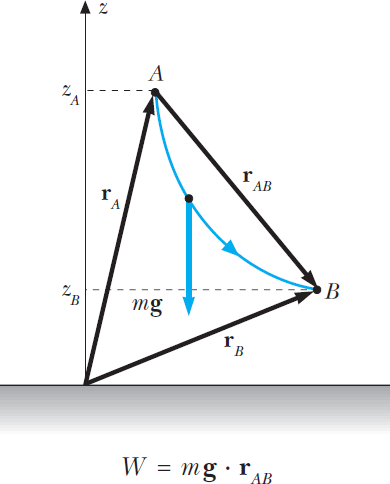
\includegraphics[width=0.3\textwidth]{Graphics-011.png}
\end{figure}
\[
    W = \int_{A}^{B} \vec F\cdot d\vec s = \vec F \int_{A}^{B} d\vec s = \vec F \cdot \vec r_{AB} = -m\vec g \cdot \vec r_{AB} = -mg(z_B - z_A) \implies -(mgz_B - mgz_A)
\]
La forza peso è una \textbf{forza conservativa}, perchè il lavoro non dipende dal percorso.
\subsection{Esempio 4.1}
Un punto di massa $m$ si trova alla base di un piano inclinato liscio; se la velocità iniziale vale $v_A$ ed è diretta come in Figura, calcolare qual è l’altezza rispetto alla base della posizione in cui il punto si ferma.\\
\begin{minipage}{0.3\textwidth}
    \centering
    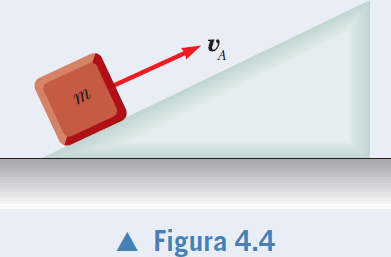
\includegraphics[width=1\textwidth]{Graphics-014.png}
\end{minipage}
\begin{minipage}{0.7\textwidth}
    \centering
    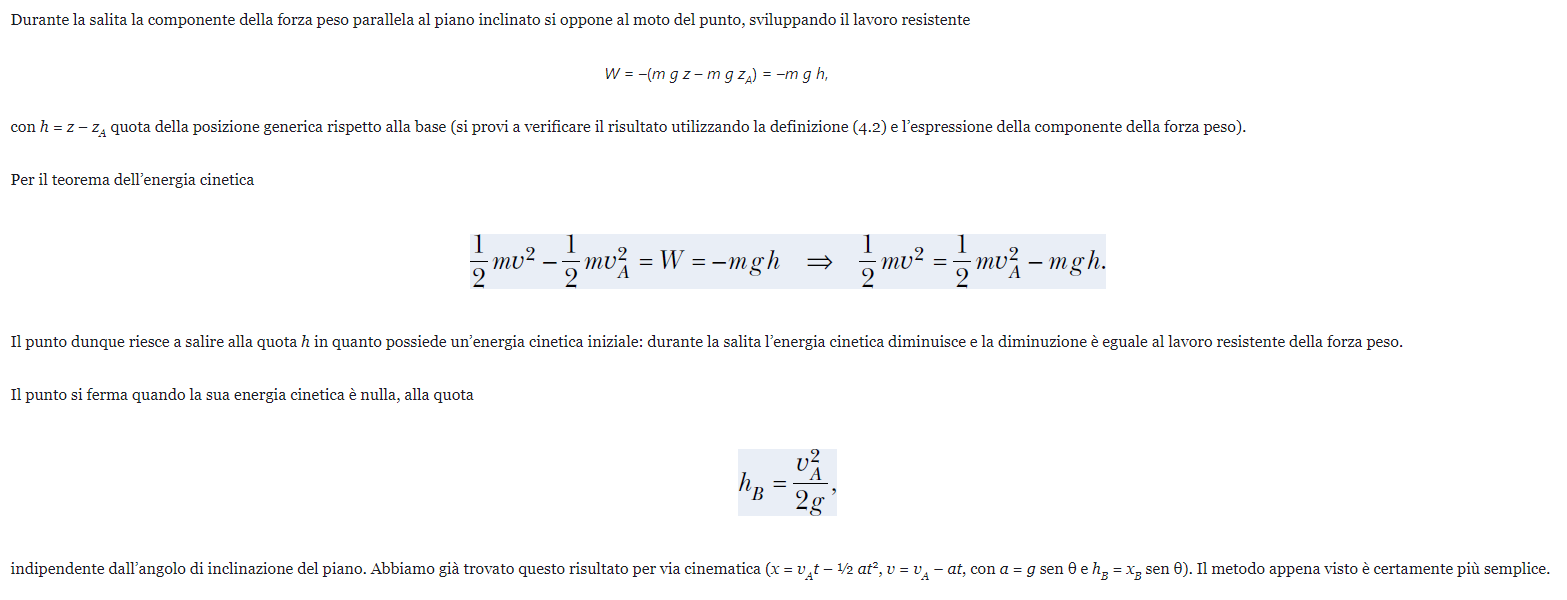
\includegraphics[width=1\textwidth]{4.1sol.png}
\end{minipage}
\subsection{Esempio 4.2}
Un punto materiale fissato a una molla di costante elastica k è in quiete nell’origine, Figura. Si applica al punto una forza $\vec F = F \vec u_x$, costante in modulo, direzione e verso, e il punto si muove lungo x. Calcolare la velocità del punto in funzione di x e la posizione in cui il punto si ferma.\\
\begin{minipage}
    {0.3\textwidth}
    \centering
    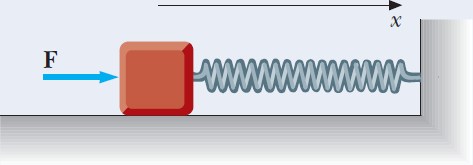
\includegraphics[width=1\textwidth]{Graphics-019.png}
\end{minipage}
\begin{minipage}{0.7\textwidth}
    \centering
    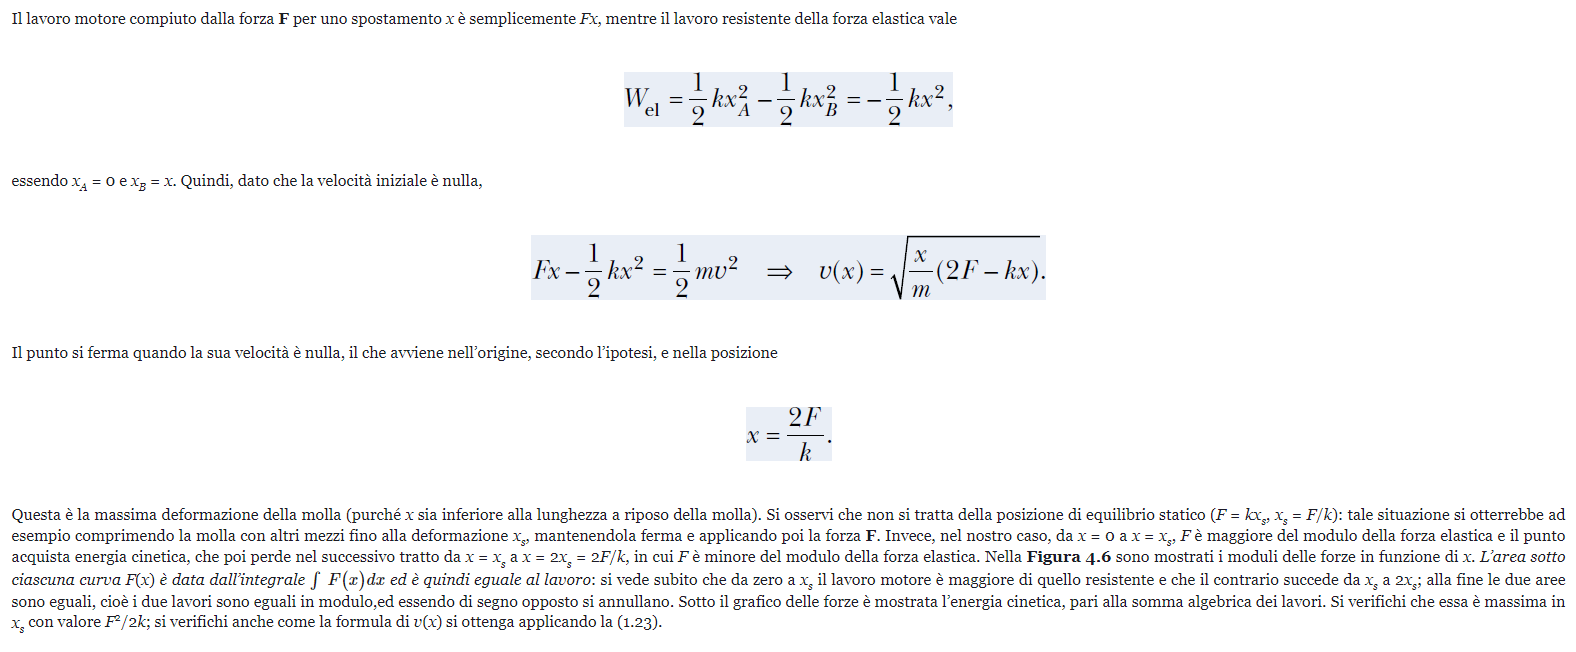
\includegraphics[width=1\textwidth]{4.2sol.png}
\end{minipage}

% vedi formula lavoro per le molle L = -((1/2)kx_b^2 - (1/2)kx_a^2)

% lavoro motore e lavoro resistente

\subsection{Esempio 4.3}

\subsection{Forze conservative}
Lavoro della forza peso:
\[
    L = -mg(h_B - h_A)
\]
Una forza è detta conservativa se il lavoro compiuto da essa non dipende dal percorso.\\
\begin{figure}[H]
    \centering
    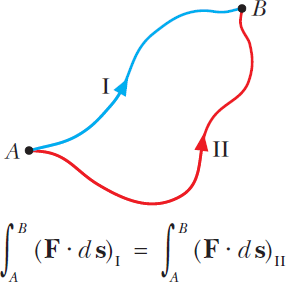
\includegraphics[width=0.2\textwidth]{Graphics-030.png}
\end{figure}
\[
    \int_{A}^{B} (\vec F \cdot d\vec s)_I = \int_{A}^{B} (\vec F \cdot d\vec s)_{II} = W_{AB}
\]
Se invece percorressi il percorso $I$ all'andata e il percorso $II$ al ritorno:
\[
    \int_{A}^{B} (\vec F \cdot d\vec s)_I = - \int_{B}^{A} (\vec F \cdot d\vec s)_{II}
\]
Di conseguenza il lavoro compiuto dalla forza $\vec F$ \textbf{lungo un percorso chiuso è nullo}:
\[
    \oint \vec F \cdot d\vec s = 0
\]
\subsection{Energia potenziale}
Se la forza è conservativa e quindi il lavoro dipende solo dalle posizioni iniziale e finale e non dal percorso, scegliendo a piacere una posizione di riferimento O nello spazio, allora il lavoro che la forza compirebbe nello spostamento tra la posizione di riferimento O e la posizione generica P:
\[
    W = \int_{O}^{P} \vec F \cdot d\vec s = - (U_P - U_O), U_O = 0 \implies = -U_P, \ E_{p,P} = - \int_{O}^{P} \vec F \cdot d\vec s
\]
\[
    W = \int_{A}^{B} \vec F \cdot d\vec s = \int_{A}^{O} \vec F \cdot d\vec s + \int_{O}^{B} \vec F \cdot d\vec s = -U_A + U_B
\]
\textbf{L'energia potenziale è la capacità di un sistema di compiere lavoro.}
\[
    L_{AB} = -\Delta U = - (U_B - U_A)
\]
Dove $U$ è l'energia potenziale ed è una funzione $U = f(x,y,z)$.
\[
    U = mgz
\]
definita a meno di una costante.
\subsubsection{Energia potenziale della forza elastica}
\[
    W_{AB} = \int_{A}^{B} kx dx = - (\dfrac{1}{2}kx_B^2 - \dfrac{1}{2}kx_A^2) \implies U = \dfrac{1}{2}kx^2
\]
quindi
\[
    W_{AB} = - \Delta U = - (U_B - U_A)
\]
\subsection{Conservazione dell'energia meccanica}
Se agiscono solo forze conservative allora l'energia cinetica sommata all'energia potenziale nel punto iniziale è uguale all'energia cinetica sommata all'energia potenziale nel punto finale:
\[
    \dfrac{1}{2}mv_B^2 - \dfrac{1}{2}mv_A^2 = - (U_B - U_A) \implies \dfrac{1}{2}mv_B^2 + U_B = \dfrac{1}{2}mv_A^2 + U_A
\]
Tale somma si chiama \textbf{energia meccanica}.\\
\textbf{Se agiscono solo forze conservative l'energia meccanica si conserva (è costante).}\\
Prendendo un corpo su un piano inclinato, la relazione rimane valida solo in assenza di attrito: se c'è attrito, possiamo ancora applicare il teorema dell'energia cinetica:
\[
    \begin{cases}
        W_c + W_{nc} = \dfrac{1}{2} mv_B^2 - \dfrac{1}{2} mv_A^2 \\
        W_c = - (U_B - U_A)                                      \\
    \end{cases}
    \implies \dfrac{1}{2} mv_B^2 - \dfrac{1}{2} mv_A^2 = - (U_B - U_A) + W_{nc} \implies (\dfrac{1}{2} mv_B^2 + U_B) - (\dfrac{1}{2} mv_A^2 + U_A) = W_{nc}
\]
Se ci sono forze non conservative abbiamo che:
\[
    E_{m_B} - E_{m_A} = W_{nc} < 0
\]


\end{document}